%----------------------------------------------------------------------------------------
%	CHAPTER 6: Economic Projections
%----------------------------------------------------------------------------------------

\chapterimage{chapter_head_6_Frankfurt.jpg} % Chapter heading image

\chapter{Business Model}

\section{Project Milestones}
Following the matrix of development per area of interest based on the funds collected during the phases of PreSale and RIPA TEC:
\begin{tcbraster}[raster columns=5,raster rows=1,raster height=0.8cm,
	valign=center, halign=center,
	enhanced,size=small,sharp corners,colframe=azure(colorwheel),coltext=white,
	colback=azure(colorwheel),fit algorithm=hybrid* ]
	\tcboxfit{}
	\tcboxfit{\textbf{25 BTC}}
	\tcboxfit{\textbf{50 BTC}}
	\tcboxfit{\textbf{250 BTC}}
	\tcboxfit{\textbf{1000 BTC}}
\end{tcbraster}
\begin{tcbraster}[raster columns=5,raster rows=4,raster height=10cm,
	valign=center, halign=center,
	enhanced,size=small,sharp corners,colframe=silver,coltext=black,
	colback=silver,fit algorithm=hybrid* ]
	\tcboxfit{\textsc{\textbf{Development}}}
	\tcboxfit{\tcbfontsize{0.8} CRYPTO $\Leftrightarrow$ CRYPTO exchange release with 25 cryptocurrencies supported and 3 main trading pairs}
	\tcboxfit{\tcbfontsize{0.8} CRYPTO $\Leftrightarrow$ FIAT exchange release with MasterCard prepaid card. 50 cryptocurrencies supported and 3 main trading pairs}
	\tcboxfit{\tcbfontsize{0.8} Advanced trading features. Open of a second and third Ripa Exchanges to join the Ripa network}
	\tcboxfit{\tcbfontsize{0.8} Open of ten Ripa Exchanges across the globe}

	\tcboxfit{\textsc{\textbf{Marketing}}}
	\tcboxfit{\tcbfontsize{0.8} Support from one agency, adv campaigns on targeted channels}
	\tcboxfit{\tcbfontsize{0.8} Support from two agencies, adv campaigns pushing harder, store with RipaEx gadgets}
	\tcboxfit{\tcbfontsize{0.8} International presentation event in London}
	\tcboxfit{\tcbfontsize{0.8} Support from five agencies, targeting all UN countries, presentation event in Tokyo}

	\tcboxfit{\textsc{\textbf{Legal}}}
	\tcboxfit{\tcbfontsize{0.8} Legal department working on AML/KYC international standards}
	\tcboxfit{\tcbfontsize{0.8} Legal departments working on AML/KYC international standards in various locations around the Globe}
	\tcboxfit{\tcbfontsize{0.8} Open of office in New York}
	\tcboxfit{\tcbfontsize{0.8} Open of office in Tokyo, intergovernmental parnership for defining AML/KYC standards}

	\tcboxfit{\textsc{\textbf{Blockchain}}}
	\tcboxfit{\tcbfontsize{0.8} DevNET development for RLSP and future ARK releases}
	\tcboxfit{\tcbfontsize{0.8} Contributions to ARK development for AVM}
	\tcboxfit{\tcbfontsize{0.8} Contributions to ARK development for standard timing releases}
	\tcboxfit{\tcbfontsize{0.8} Partnership with ARK for blockchain technology developments}
\end{tcbraster}

\section{Market Overview}
	\subsection{Cryptocurrency Market Size and Technology}
		\begin{itemize}
			\item The cryptocurrency market cap has been projected to reach as high as 
			\href{https://www.ccn.com/cryptocurrency-market-cap-to-reach-2-trillion-in-2018-mike-novogratz/}{\$1-2 trillion in 2018}
			\cite{novograzPrediction}.
			\item The market cap of Bitcoin exceeded \href{https://coinmarketcap.com/currencies/bitcoin/historical-data/}{\$70 billion}
			\cite{coinmarketcapHistorical}, 
			with peak trading volumes around \$3 billion per day.
			\item Technology consulting firm CB Insights has identified \href{https://www.cbinsights.com/blog/industries-disrupted-blockchain/}{27 ways} 
			\cite{cbinsights} blockchain can fundamentally change processes as diverse as banking, cybersecurity, voting, and academics.
			\item The World Economic Forum estimates that by 2027, 
			\href{http://www3.weforum.org/docs/WEF_GAC15_Technological_Tipping_Points_report_2015.pdf}{10\% of global GDP} \cite{wefTTP} 
			will be stored on blockchain technology.
			\item Most mining pools are located in China, comprising 
			\href{https://www.buybitcoinworldwide.com/mining/china/}{more than 70\%} \cite{bitcoinMiningChina}
			of total Bitcoin mining. China manufactures most cryptocurrency mining equipment and leverages the country’s cheap electricity prices.
		\end{itemize}
		\begin{center}
			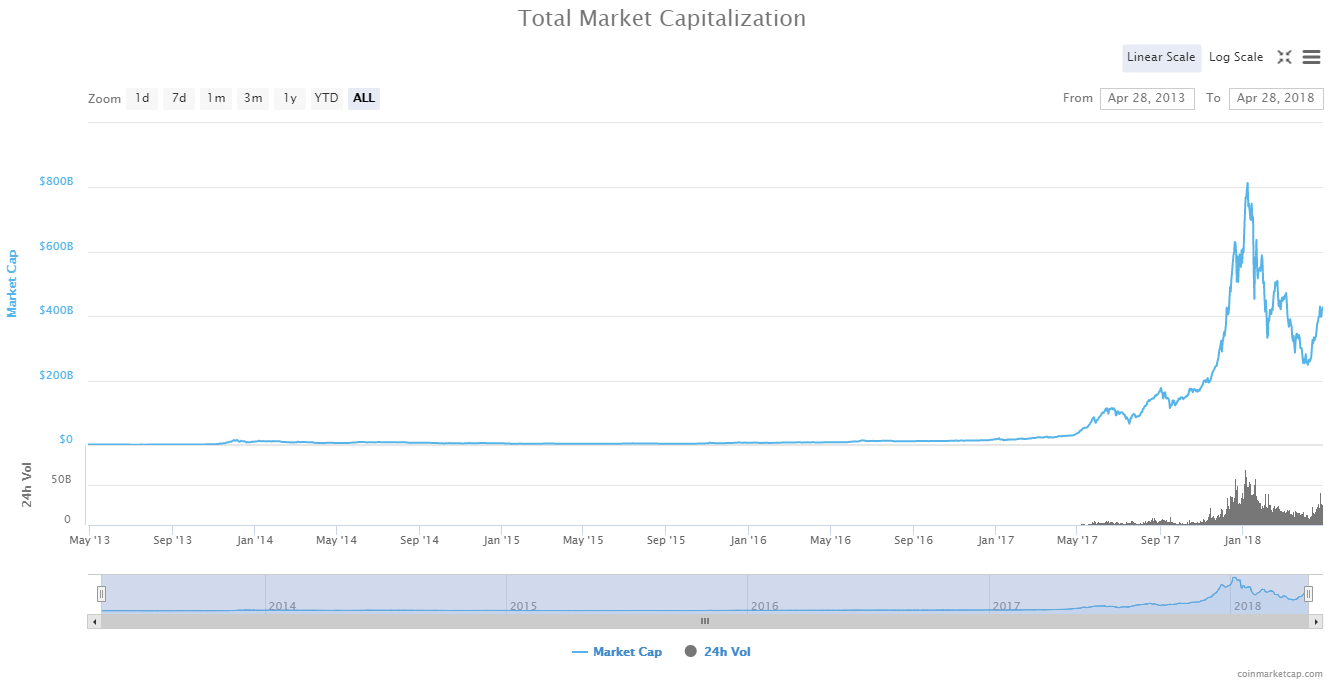
\includegraphics[width=\textwidth,height=\textheight,keepaspectratio]{CryptoMarketCap}
			\captionof{figure}{Cryptocurrency market capitalization April 2018}
		\end{center}

	\subsection{Types of Cryptocurrencies}
		\begin{itemize}
			\item There are \href{https://coinmarketcap.com/all/views/all/}{over 1,000 cryptocurrencies} \cite{coinmarketcapAll} 
			in existence right now (called ``altcoin''); 
			over 600 have market capitalizations of over \$100,000.
			\item While Bitcoin’s price has generally been following upward trend, in early 2018, Bitcoin’s price fell sharply, 
			\href{https://www.cnbc.com/2018/02/05/bitcoin-price-drops-below-8000-over-60-billion-wiped-off-cryptocurrencies.html}{dipping below \$8,000} 
			\cite{cnbcBitcoinPriceSurge}
			as news of tougher regulation from China and South Korea surfaced. Bitcoin's price also fell 
			following announcements of \href{http://www.latimes.com/business/la-fi-bitcoin-sec-registration-20180307-story.html}{SEC crackdown} 
			\cite{laTimes}
			on crypto exchanges and after Binance 
			\href{https://www.ft.com/content/58a32050-22aa-11e8-add1-0e8958b189ea}{was reportedly hacked}
			\cite{ftBinanceHack}.
			\item Bitcoin’s market share has fallen from 81\% in June 2016 to 41\% one year later, in June 2017. 
			However, Bitcoin’s price has continued to soar.
			\item In August 2017, Ether’s market capitalization was around \$28 billion. At one point, 
			\href{http://www.zerohedge.com/news/2017-05-31/ethereum-forecast-surpass-bitcoin-2018}{commentators} \cite{zeroHedge}
			anticipated that Ether’s market 
			capitalization would surpass that of Bitcoin (the 
			\href{https://www.flippening.watch/}{``flippening''} \cite{flippening}). 
			However, issues with Ethereum technology have since caused its value to decline.
		\end{itemize}
		\begin{center}
			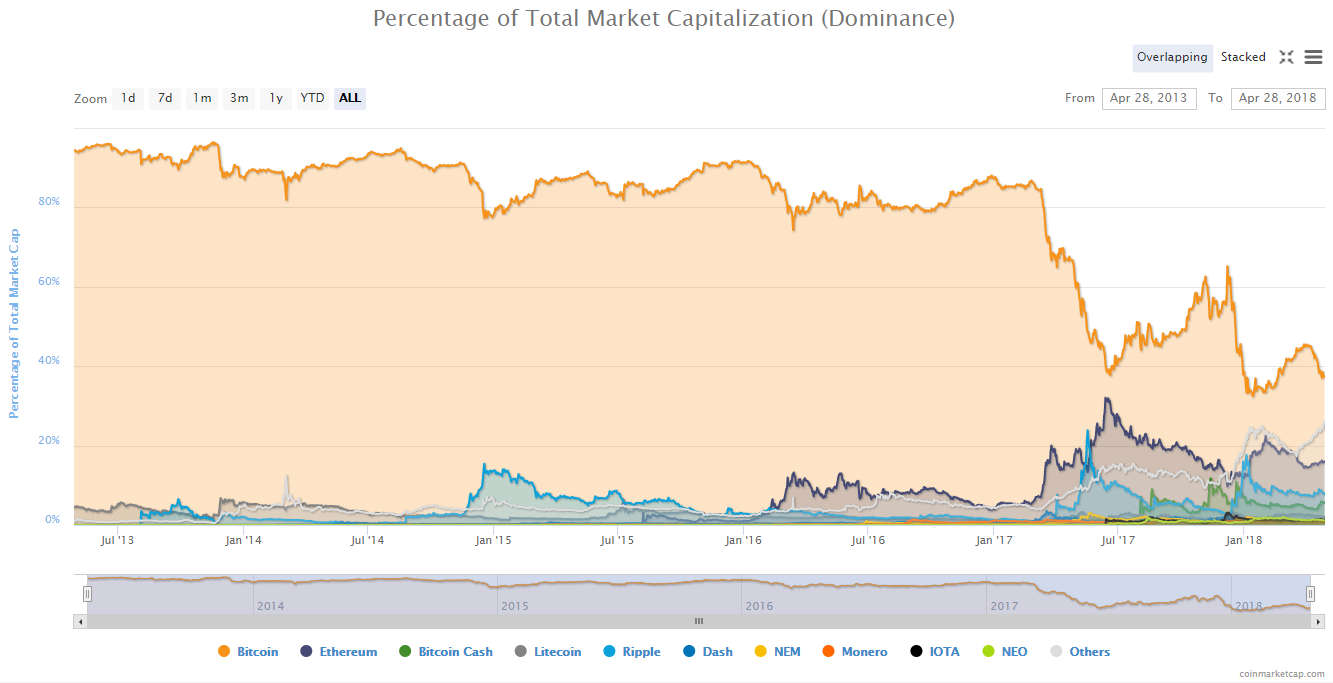
\includegraphics[width=\textwidth,height=\textheight,keepaspectratio]{CryptoMarketDominance}
			\captionof{figure}{Cryptocurrency market dominance April 2018}
		\end{center}

	\subsection{Investing in Cryptocurrencies}
		\begin{itemize}
			\item Supply and demand matters. The rate of increase of the supply of Bitcoin will decrease until the number 
			of Bitcoin reaches 21 million, 
			\href{https://www.coindesk.com/top-10-bitcoin-myths-debunked/}{which is expected to take place in the year 2140}
			\cite{mythsDebunked}. Similarly, 
			the supply of Litecoin will be capped at 
			\href{https://support.xbtce.info/Knowledgebase/Article/View/152/59/about-litecoin}{84 million units}
			\cite{ltcLimits}.
			\item Initial coin offerings are trending right now. This year, former Mozilla CEO Brendan Eich raised \$35 
			million from an ICO in 
			\href{https://techcrunch.com/2017/06/01/brave-ico-35-million-30-seconds-brendan-eich/}{less than 30 seconds}
			\cite{techCrunch}, 
			and Bancor Protocol raised \$153 million in 
			\href{https://www.google.com/search?q=Bancor+Protoco+ico&oq=Bancor+Protocol+ico&gs_l=psy-ab.3..0i13k1l2.253.542.0.578.4.3.0.0.0.0.177.320.0j2.2.0....0...1.1.64.psy-ab..3.1.176.LOjRpj0hKrM}{under three hours}
			\cite{bancorProtocol}.
			\item Blockchain-related projects have raised more than 
			\href{https://www.coindesk.com/1-6-billion-all-time-ico-funding-climbs-as-record-500-million-invested-in-july/}{\$1.6 billion via ICOs} 
			\cite{coindeskICOAllTimeHigh} 
			to date, while venture capitalists have provided only 
			\href{http://my.pitchbook.com/?pbr=14763750}{\$550 million} \cite{pitchbook} for cryptocurrency companies.
		\end{itemize}
		\begin{center}
			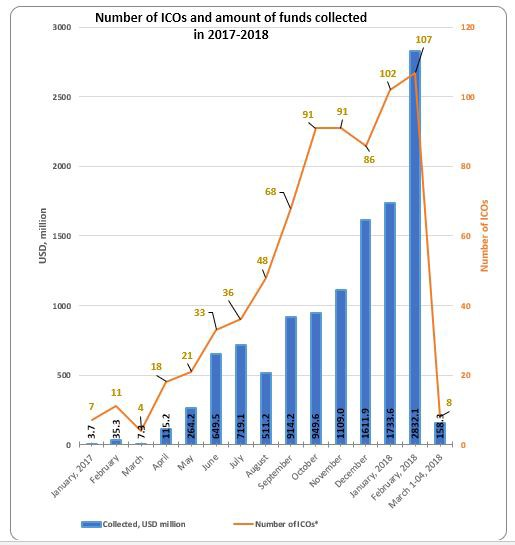
\includegraphics[width=\textwidth,height=\textheight,keepaspectratio]{FundsCollectedICO}
			\captionof{figure}{Funds colleted in ICOs in 2017-2018}
		\end{center}

	\subsection{Outstanding Issues}
		\begin{itemize}
			\item \textbf{Accounting}. While the US has been cracking down on unregulated activities, in countries such as 
			\href{https://techcrunch.com/2013/08/19/germany-recognizes-bitcoin-as-private-money-sales-tax-coming-soon/}{Germany} 
			\cite{techCrunchPrivateMoney}
			and the \href{http://www.ibtimes.co.uk/hmrc-re-classify-bitcoin-private-money-1432718}{UK}
			\cite{ibtimesPrivateMoney}, 
			cryptocurrencies are treated like ``private money'' and are not subject to tax outside of commercial use.
			\item \textbf{Regulation}. New York State created the 
			\href{https://www.wired.com/2014/07/ny_bitcoin/}{BitLicense system} \cite{wiredNYLicense}, mandates for companies 
			before conducting business with New York residents. As of mid-2017, only three BitLicenses have been issued, 
			and a far greater number withdrawn or denied. In Asia, where cryptocurrency demand has been soaring, 
			the \href{http://fortune.com/2018/01/17/china-bitcoin-cryptocurrency-crackdown/}{Chinese} 
			\cite{fortune}
			and \href{https://www.bloomberg.com/news/articles/2017-12-13/south-korea-seeks-measures-to-curb-frenzied-bitcoin-speculation}{South Korean} 
			\cite{bloombergSKBan}
			governments have taken hard stances on cryptocurrency regulation.
			\item \textbf{Security}. The 
			\href{https://www.forbes.com/sites/laurashin/2016/12/20/hackers-have-stolen-millions-of-dollars-in-bitcoin-using-only-phone-numbers/#3ac0bf1d38ba}{FTC recorded} 
			\cite{forbesBitcoinHacking} 
			an increase in identity fraud complaints of more than 100\% between 2013 and 2016, 
			and Coinbase, the largest US-based exchange, saw account hacking double just between November and December 2016.
		\end{itemize}

\section{Local Market Analysis and 5 Years Projection}
Ripa Exchange on its opening at the beginning of next year and for all the year 2019 is to be expected
to have the following operating numbers:
\begin{itemize}
	\item Registered Users: 5,000			%(1,600,000 BitFinex, 40,000 TheRockTrading)
	\item 24/hours Volume: 25 BTC			%(50,000 BTC BitFinex, 100 BTC TheRockTrading)
	\item Monthly Volume: 750 BTC			%(2,000,000 BTC BitFinex, 5,000 BTC TheRockTrading)
\end{itemize}

Given a transaction fee of 0.20\% the revenue for the first year of operation are expected to be in the order of 180 BTC the 
outcome for the years 2 to 5 is expected to be in the rage described in figure \ref{fig:fiveYearsProjection} 
\begin{center}
	\begin{tikzpicture}
		\begin{axis}[
			symbolic x coords={2019, 2020, 2021, 2022, 2023},
			xtick=data,
			ylabel=BTC,
			xlabel=years
		]
			\addplot[ybar,fill=azure(colorwheel)] coordinates {
				(2019, 180)
				(2020, 300)
				(2021, 500)
				(2022, 1000)
				(2023, 2000)
			};
			\addplot+ [
				sharp plot, color=silver, mark=diamond
				] coordinates {
				(2019,180) (2020,300) (2021,500) (2022,1000) (2023,2000)
				};			
		\end{axis}	
	\end{tikzpicture}
	\captionof{figure}{5 years revenue projection}
	\label{fig:fiveYearsProjection}
\end{center}

Depending on the closing value of the RipaEx ICO, the project is to be expected to open N.1 to N.9 others Ripa Exchange in 
the biennium 2019-2020 spreading the use of the Ripa Exchange codebase and the usage of the XPX token associated with the 
Ripa Blockchain making the figure above into account for each single Ripa Exchange installation.

\section{XPX Token Economics}
As explained in section \ref{sec:theRipaBlockchain} the Ripa Blockchain will have its own XPX token (\PHP symbol) that 
will serve the following purposes:
	\begin{enumerate}
		\item to list new cryptocurrencies on Ripa Exchanges
		\item to advertise new projects
		\item to buy RipaEx gadget on RipaEx Store
		\item to pay for the sell of goods \& services on authorized resellers with our RipaEx POS (Point of Sale)
		\item to share liquidity between Ripa Exchanges in the same network
	\end{enumerate}
It is our main purpose that the economy of the XPX token will stay healthy for all the duration of the RipaEx project for 
this reason we will apply economic strategies\footnote{Like burning tokens not covered from ICO funds} 
to the token economy to make the price of the token rise constantly during all the duration of the project and beyond.

